\subsection{PID Controller}\label{section:pid_controller}
\subsubsection{Basic Structure}
The PID controller generates a control signal $u(t)$ based on the error signal $e(t)$, which is the difference between the desired setpoint and the measured process variable (see Fig. \ref{fig:control-loop-block-diagram}). The control signal is computed as:

\begin{equation}
	u(t) = K_p e(t) + K_i \int_0^t e(\tau)d\tau + K_d \frac{d}{dt}e(t)
\end{equation}

Where:
\begin{itemize}
	\item $u(t)$: Control signal applied to the system.
	\item $e(t)$: Error signal, representing the deviation from the setpoint.
	\item $K_p$: Proportional gain, which responds to the current error.
	\item $K_i$: Integral gain, which addresses accumulated past errors.
	\item $K_d$: Derivative gain, which predicts future error trends based on the rate of change.
\end{itemize}

\subsubsection{Discrete Time Implementation}
For digital implementation, the continuous-time PID equation is discretized to suit microcontroller-based systems. The discrete-time PID control signal u[n]u[n] is calculated as:

\begin{equation}
	u[n] = K_p e[n] + K_i T_s \sum_{k=0}^n e[k] + K_d \frac{e[n] - e[n-1]}{T_s}
\end{equation}

where:
\begin{itemize}
	\item $T_s$: Sampling period, representing the time interval between consecutive control updates.
	\item $e[n]$: Error signal at the nn-th sampling instant.
	\item $u[n]$: Control signal at the nn-th sampling instant.
\end{itemize}
This formulation ensures compatibility with real-time embedded systems while maintaining control precision.


\subsection{Tuning Methodology}
The Ziegler-Nichols method is a widely used and systematic approach for tuning PID controllers. It provides a reliable framework for determining initial controller parameters, which can then be fine-tuned for optimal performance. The method involves inducing controlled oscillations in the system to identify critical parameters, which are then used to calculate the proportional, integral, and derivative gains.
\subsubsection{Ziegler-Nichols Method}
The Ziegler-Nichols tuning procedure consists of the following steps:
\begin{enumerate}
	\item \textbf{Initialize Parameters}: Set the integral gain \( K_i \) and derivative gain \( K_d \)to zero, leaving only the proportional gain \( K_p \) active.
	\item \textbf{Induce Oscillations}: Gradually increase \( K_p \) until the system exhibits sustained oscillations. At this point, the system is at the threshold of stability, and the proportional gain is referred to as the ultimate gain \( K_u \). The period of these oscillations is denoted as \( T_u \).
	\item \textbf{Record Critical Values}: Note the values of \( K_u \) and \( T_u \), as they are essential for calculating the final PID parameters.
	\item \textbf{Calculate PID Gains:} Using the recorded values, compute the PID parameters as follows:
	\begin{equation}
		\begin{aligned}
			K_p &= 0 . 6K_u \\
			T_i &= 0 . 5T_u \\
			T_d &= 0 . 125T_u  \label{eq:eq}
		\end{aligned}
	\end{equation}
	Here, \( T_i \) and \( T_d \) represent the integral and derivative time constants, respectively. These values are then used to determine the integral and derivative gains:
	\begin{equation}
		\begin{aligned}
			K_i = \frac{K_p}{T_i} \quad \text{and} \quad K_d = K_p \cdot T_d.  \label{eq:eq}
		\end{aligned}
	\end{equation}
\end{enumerate}

This method provides a robust starting point for achieving stable control. However, it is important to note that the Ziegler-Nichols method may require additional fine-tuning to account for system-specific dynamics and performance requirements. The calculated parameters serve as an initial baseline, which can be further optimized through iterative testing and adjustment.


\subsubsection{Practical Tuning Guidelines}
In addition to the Ziegler-Nichols method, practical tuning guidelines were applied to refine the controller performance:

\begin{itemize}
	\item Start with a small proportional gain $K_p$ (e.g. $K_p$ = 10) to avoid instability.
	\item Introduce the derivative term $K_d$ to dampen oscillations, typically setting $K_d = 0 . 1K_p$.
	\item  Fine-tune $K_p$, $K_i$, and $K_d$ iteratively to achieve optimal stability and responsiveness.
\end{itemize}


\subsection{Cascaded PID Control Strategy}
To optimize system performance and resource utilization, the control loop employs a cascaded PID strategy:
\begin{itemize}
	\item \textbf{Pitch Control}: Updated at the highest frequency (e.g., every control cycle) to ensure rapid response to changes in the robot's tilt and maintain balance.
	\item \textbf{Yaw and Position Control}: Updated at a lower frequency (e.g., every 8th cycle) to reduce computational load while still providing adequate motion control.
\end{itemize}

This approach prioritizes critical tasks (e.g., maintaining balance) while efficiently managing system resources, ensuring robust and stable operation. A simplified block diagram for a cascaded PID controller is shown in Fig.~\ref{fig:control-loop}

\begin{figure}[H]
	\centering
	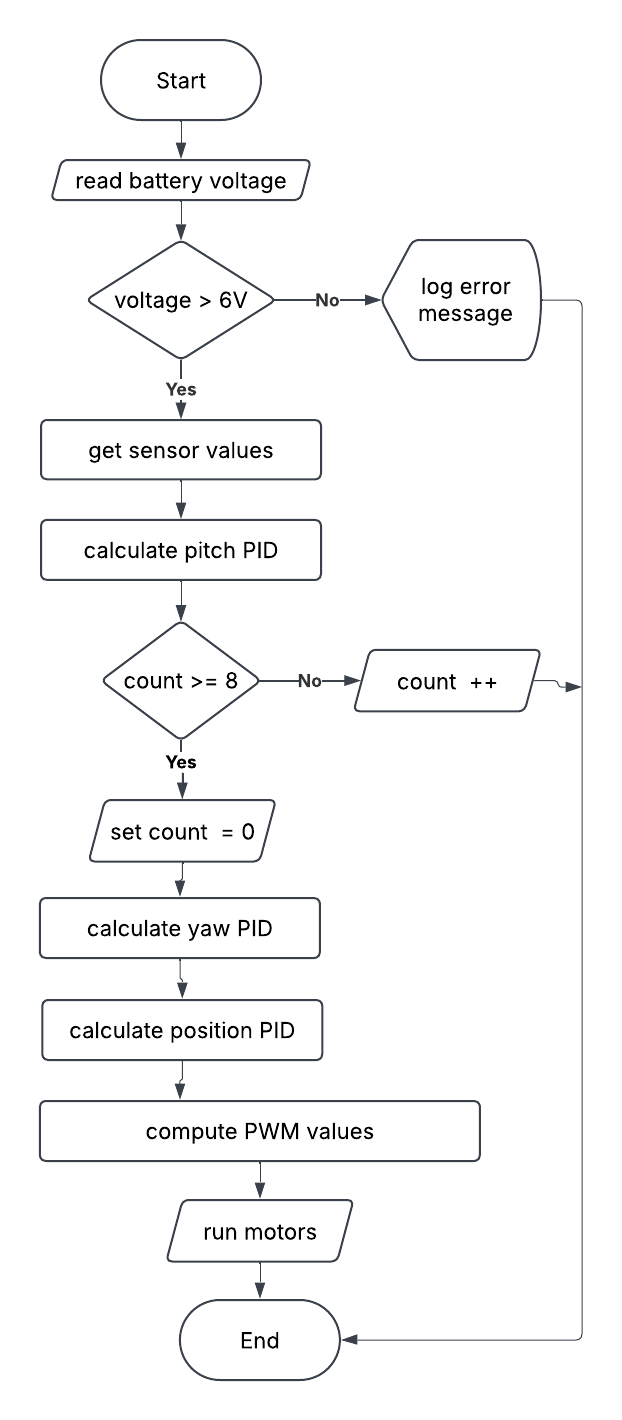
\includegraphics[width=0.5\linewidth]{assets/control_loop_diagram.png}
	\caption{A simplified block diagram of the cascaded control loop used. }
	\label{fig:control-loop}
\end{figure}

\subsubsection{Pitch PID Control:}
The pitch control loop ensures the robot maintains its upright position. The primary objective of the pitch controller is to minimize the deviation of the robot's pitch angle from a set-point, which is ideally zero degrees (i.e., upright). The pitch control output is calculated using the PD algorithm, where the error is the difference between the current pitch angle and the desired pitch angle. 
\begin{equation}
	\tau_{\theta,pid} = K_{p\theta}({\theta_{desired} - \theta_{measured}}) + K_{d\theta}\frac{d}{dt}(\theta_{desired} - \theta_{measured})
\end{equation}

Below is its code implementation:
\begin{lstlisting}[style=cppstyle2]
	inline void runPitchControl() {
		pitch_pid_output = (kp_balance * (kalman.angle - 0)) + (kd_balance * gyro_x);
	}
\end{lstlisting}

The final results are shown in Fig.~\ref{fig:pid_position_kp_55_kd_1_25}.
\begin{figure}[H]
	\centering
	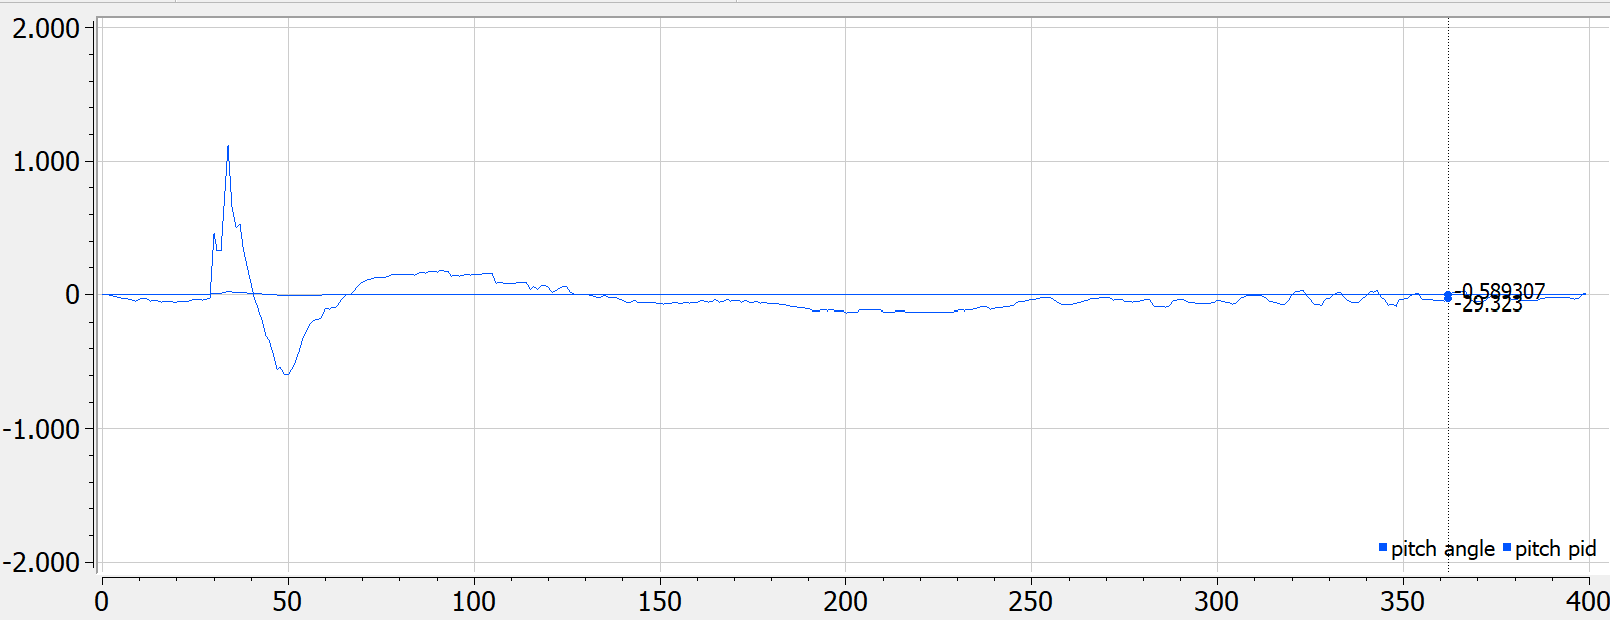
\includegraphics[width=0.8\linewidth]{assets/pid_pitch_kp_55_kd_1_25.png}
	\caption{Pitch angle control system response at $K_{p\theta}$ = 55 and $K_{d\theta}$ = 1.25. The data was recorded at baud rate of 115200.}
	\label{fig:pid_position_kp_55_kd_1_25}
\end{figure}

\textbf{Eliminating Jitter}:
Once the system reaches stability, it begins to exhibit jitter (i.e. small, rapid fluctuations in the control output), as observed in the PID output between data points 250 and 400 in Fig.~\ref{fig:pid_position_kp_55_kd_1_25}. This jitter arises due to the high sensitivity of the derivative gain ($K_{d\theta}$) to fluctuations in the gyroscope readings ($\dot{\theta}$). While reducing $K_{d\theta}$ mitigates the jitter, it also diminishes the system's ability to dampen oscillations, leading to excessive overshoot and potential instability. Fig.~\ref{fig:pid_position_overshoot} illustrates the system's response when using $K_{p\theta}$ = 55 and $K_{d\theta}$ = 0.75 where significant overshoot is evident.

\begin{figure}[H]
	\centering
	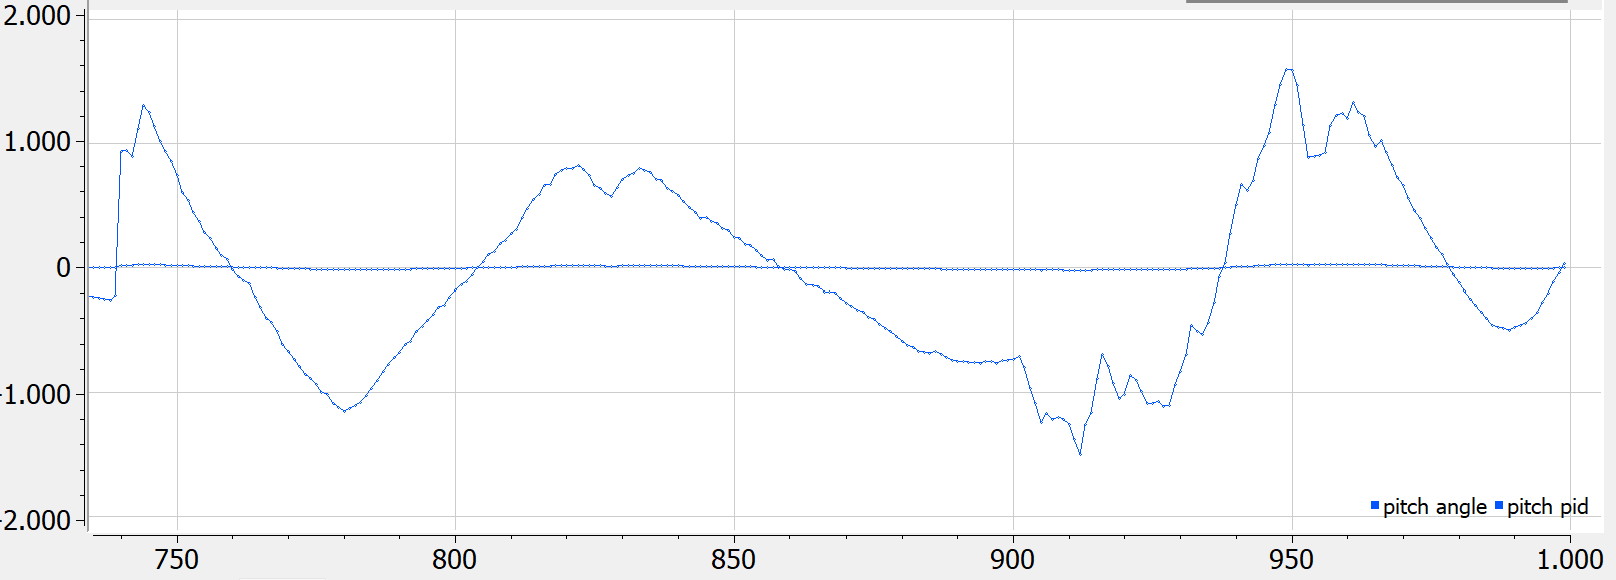
\includegraphics[width=0.7\linewidth]{assets/pid_pitch_overshoot.png}
	\caption{Pitch angle control system response at $K_{p\theta}$ = 55 and $K_{d\theta}$ = 0.75. Data recorded at baud rate of 115200.}
	\label{fig:pid_position_overshoot}
\end{figure}

To address this issue, an \textbf{adaptive derivative gain approach} is implemented, where $K_{d\theta}$ is adjusted dynamically based on the pitch angle of the robot. When the absolute pitch angle exceeds a predefined threshold, a higher derivative gain is used to provide stronger correction, while a lower gain is applied for small angles to minimize jitter. The corresponding implementation is as follows:
\begin{lstlisting}[style=cppstyle2]
	if (pitch_angle > 8) { kd_balance = kd_balance_large_angle; }
	else { kd_balance = kd_balance_small_angle; }
	
	inline void runPitchControl() {
		pitch_pid_output = (kp_balance * (kalman.angle - 0)) + (kd_balance * gyro_x);
	}
\end{lstlisting}

This adaptive control strategy effectively stabilizes the system while reducing excessive oscillations. Fig.~\ref{fig:pid_position_combined} presents the improved system response, demonstrating a smoother transition and enhanced overall stability.
\begin{figure}[H]
	\centering
	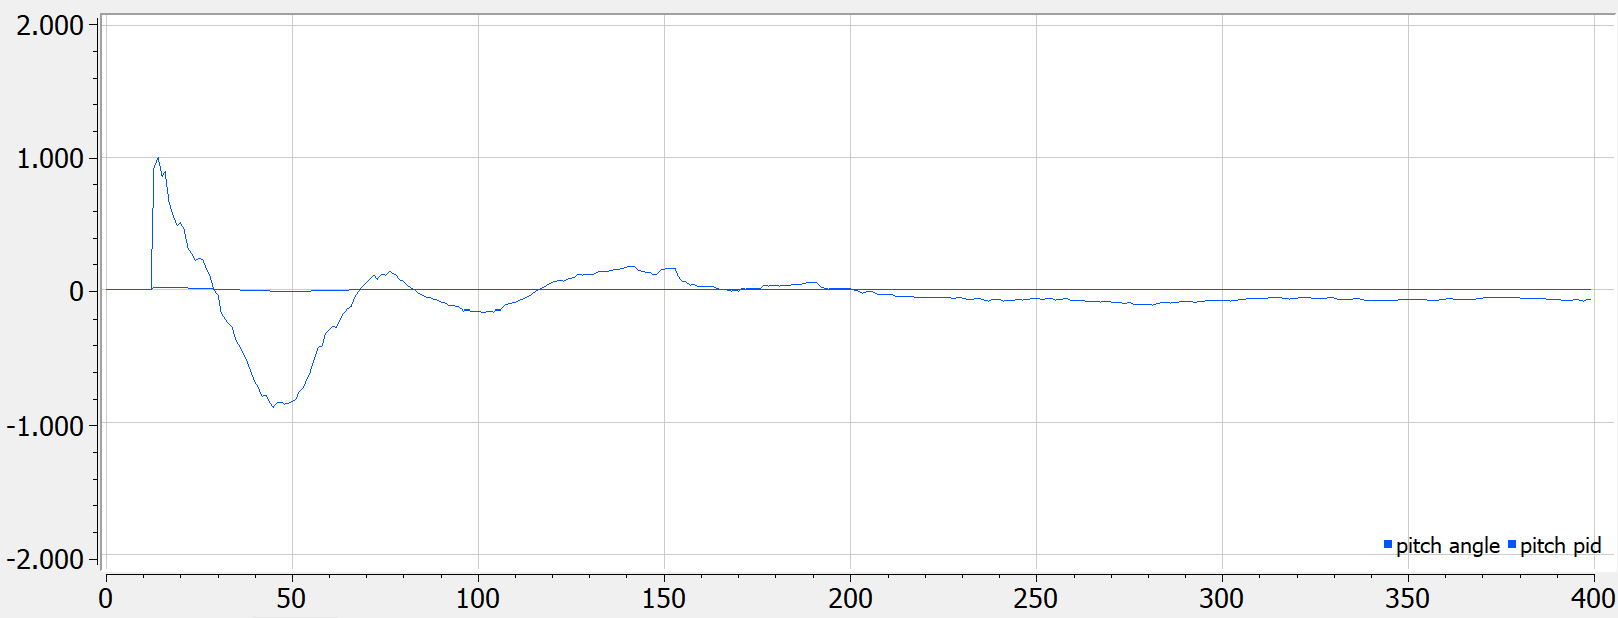
\includegraphics[width=0.8\linewidth]{assets/pid_pitch_combined.png}
	\caption{Pitch angle control system response. The data was recorded at baud rate of 115200.}
	\label{fig:pid_position_combined}
\end{figure}


\subsubsection{Yaw Control:}
Yaw control is responsible for controlling the robot's rotational movement around its vertical axis. The yaw PID controller computes the control output based on the robot's angular velocity, which is measured by the gyroscope along the z-axis. 
\begin{equation}
	\tau_{\phi,pid} = K_{p\phi}(\phi_{desired} - \phi_{measured}) + K_{d\phi}\frac{d}{dt}(\phi_{desired} - \phi_{measured})
\end{equation}

Below is its code implementation:
\begin{lstlisting}[style=cppstyle2]
	inline void runYawControl(){
		float delta_yaw_angle = yaw_angle_degrees - desired_yaw_angle;
		yaw_pid_output = (kp_turn * delta_yaw_angle) + (kd_turn * gyro_z);
	}
\end{lstlisting}

The yaw control adjusts the motor speeds to achieve the desired angle, ensuring the robot maintains a stable heading. Fig.~\ref{fig:pid_yaw} illustrates the system's response with \(K_{p\phi}\) = 2.5 and $K_{i\phi}$ = 0.5 when transitioning from an initial angle of $-20 \ deg$ to final angle of $+20 \ deg$.
\begin{figure}[H]
	\centering
	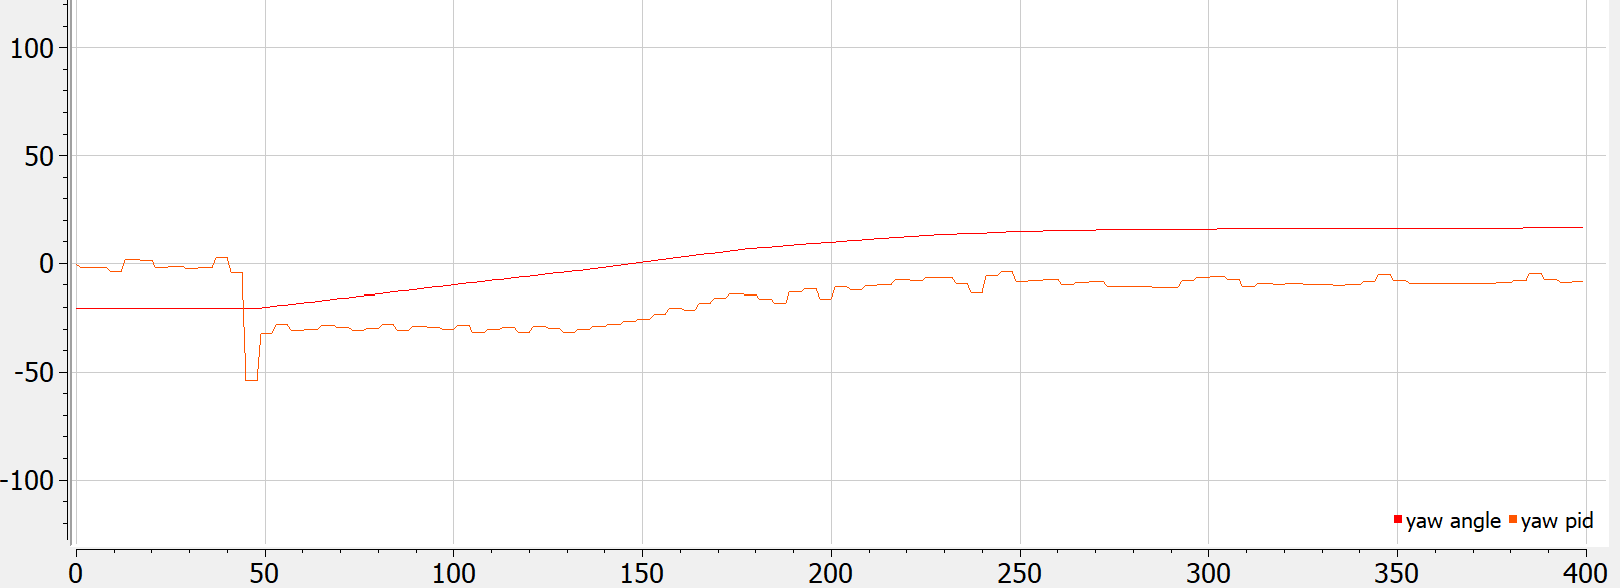
\includegraphics[width=0.8\linewidth]{assets/pid_yaw_kp_2_5_kd_0_5_target_20_deg.png}
	\caption{Yaw angle control system response at \(K_p\) = 2.5 and $K_i$ = 0.5 for an angle transition from $-20 \ deg$ to $+20 \ deg$. The data was recorded at baud rate of 115200.}
	\label{fig:pid_yaw}
\end{figure}

\subsubsection{Position Control:}
Position control is implemented to ensure the robot moves smoothly and accurately along a path or to a target location. The encoder feedback from the left and right wheels is used to calculate the robot's displacement and speed. The position PID controller adjusts the motor speeds to minimize the error in position and velocity.
\begin{equation}
	\tau_{x,pid} = K_{px}(x_{desired} - x_{measured}) + K_{dx}\frac{d}{dt}(x_{desired} - x_{measured})
\end{equation}

Below is its code implementation:
\begin{lstlisting}[style=cppstyle2]
	inline void runPositionControl(){
		position_pid_output = - (kp_position * (current_position - move_to_position)) - (kd_position * encoder_speed_filtered);
	}
\end{lstlisting}

The position controller continuously adjusts motor speeds to reduce position error while maintaining a stable heading. Fig.~\ref{fig:pid_postition} presents the system's response when \(K_{px}\) = 0.26 and $K_{dx}$ = 20 when moving from relative distance of $-60 \ cm$ to $+30 \ cm$.
\begin{figure}[H]
	\centering
	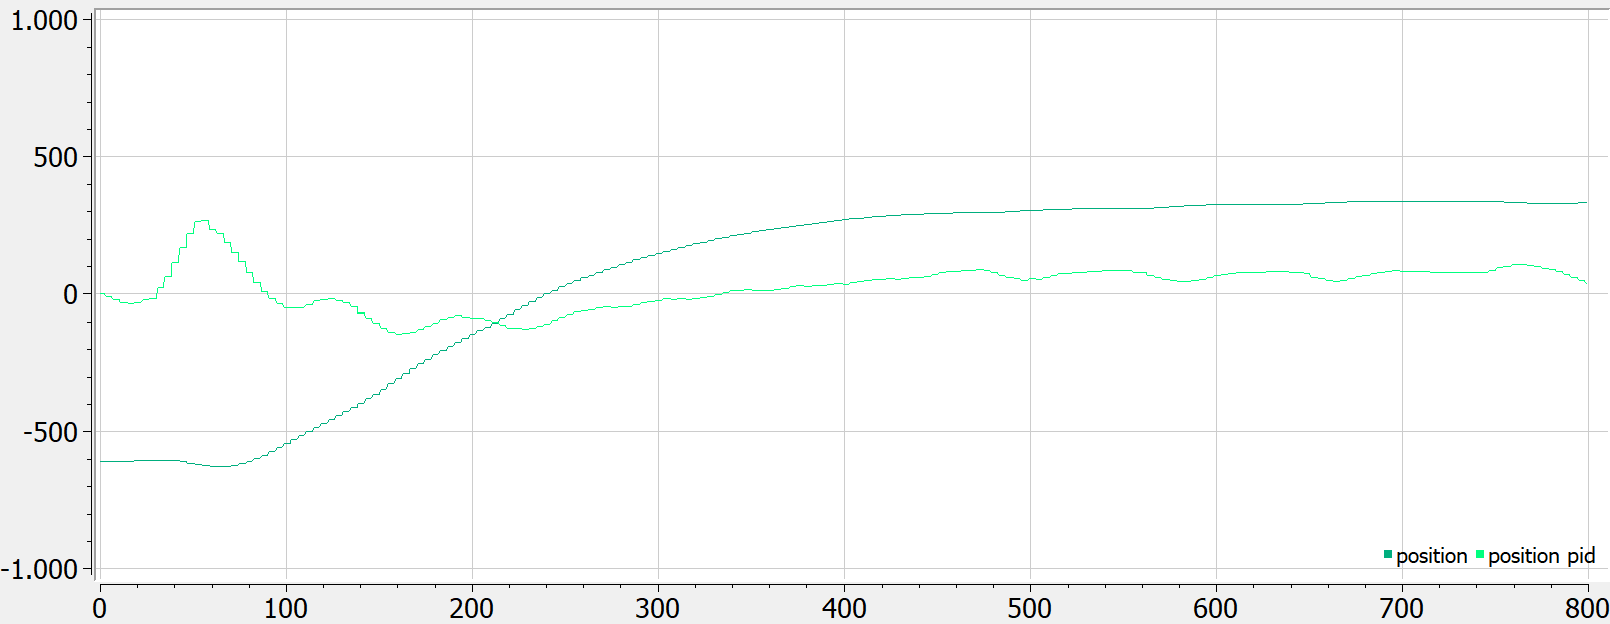
\includegraphics[width=0.8\linewidth]{assets/pid_position_kp_0_26_kd_20.png}
	\caption{Position control system response with \(K_{px}\) = 0.26 and $K_{dx}$ = 20 for a displacement of $-60 \ cm$ to $+30 \ cm$. Data recorded at baud rate of 115200.}
	\label{fig:pid_postition}
\end{figure}


\subsubsection{Combining Control Outputs}
The final motor control is achieved by combining the outputs from all three PID controllers. The outputs from the pitch, yaw, and position PID controllers are used to calculate the motor speeds, which determine the robot's motion. Specifically, the following equation is used to compute the PWM values for the left and right motors:

\begin{align}
	\tau_{left,motor} &= \tau_{\theta,pid} - \tau_{\phi,pid} - \tau_{x,pid} \\
	\tau_{right,motor} &= \tau_{\theta,pid} + \tau_{\phi,pid} - \tau_{x,pid}
\end{align}

Below is its code implementation:
\begin{lstlisting}[style=cppstyle2]
	void balance(){
		...
		
		pwm_left = pitch_pid_output - yaw_pid_output - position_pid_output;
		pwm_right = pitch_pid_output + yaw_pid_output - position_pid_output;
		pwm_left = constrain(pwm_left, -255, 255);
		pwm_right = constrain(pwm_right, -255, 255);
		
		...
	}
\end{lstlisting}
The PWM values are constrained between -255 and +255 to prevent exceeding motor driver limits. Where +255 represents maximum forward speed, -255 maximum reverse, and 0 a stationary state. The computed Pulse-Width-Modulation (PWM) are transmitted to the motor drivers, which adjust the robot's movement and balance in real time. This closed-loop control mechanism ensures precise and stable operation by continuously refining motor outputs based on sensor feedback. A simplified diagram of the motor control loop is illustrated in Fig.~\ref{fig:schematics_control-loop}.

\begin{figure}[H]
	\centering
	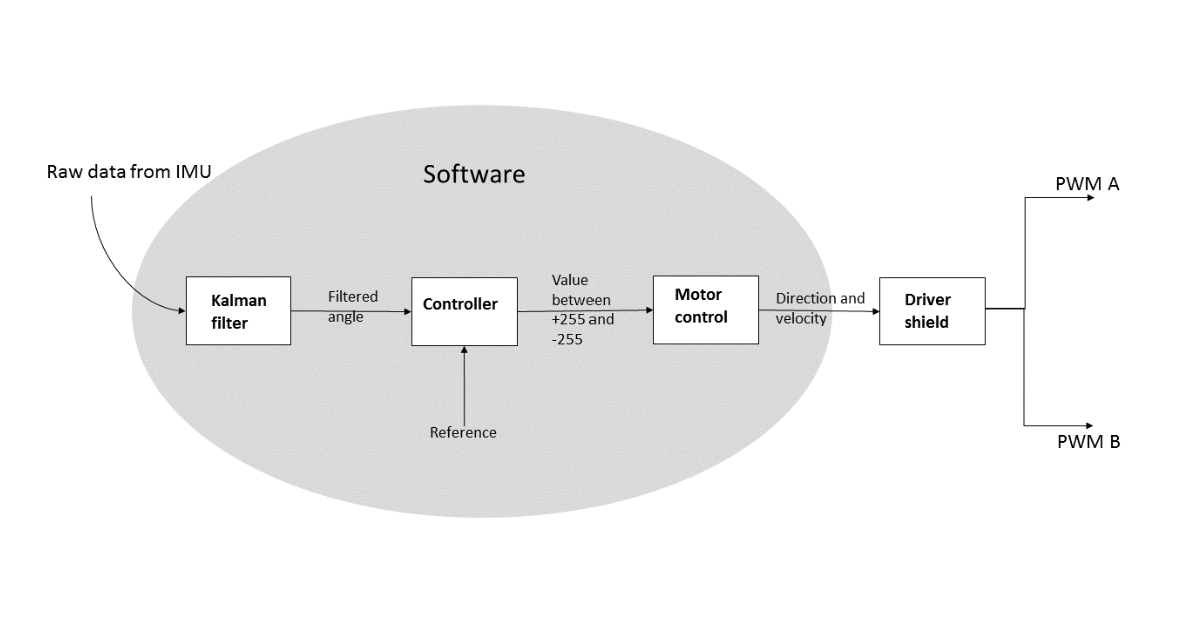
\includegraphics[height=8cm]{assets/pitch_angle_control_loop.png}
	\caption{A simplified diagram of the motor control loop \cite{10193276}.}
	\label{fig:schematics_control-loop}
\end{figure}


\subsubsection{Combined Results}
The use of PID controllers for pitch, yaw, and position control enables the robot to maintain balance and navigate effectively. The proportional, integral, and derivative terms in each PID loop allow the system to respond to real-time errors, minimize steady-state deviations, and anticipate future errors, leading to smooth and precise control of the robot's motion. The integration of these PID controllers is fundamental to the robot's stability and performance. The complete flow chart is shown in Fig.~\ref{fig:code-overview-flowchart} and the combined results are shown in Fig.~\ref{fig:final_pid}

\begin{figure}[h]
	\centering
	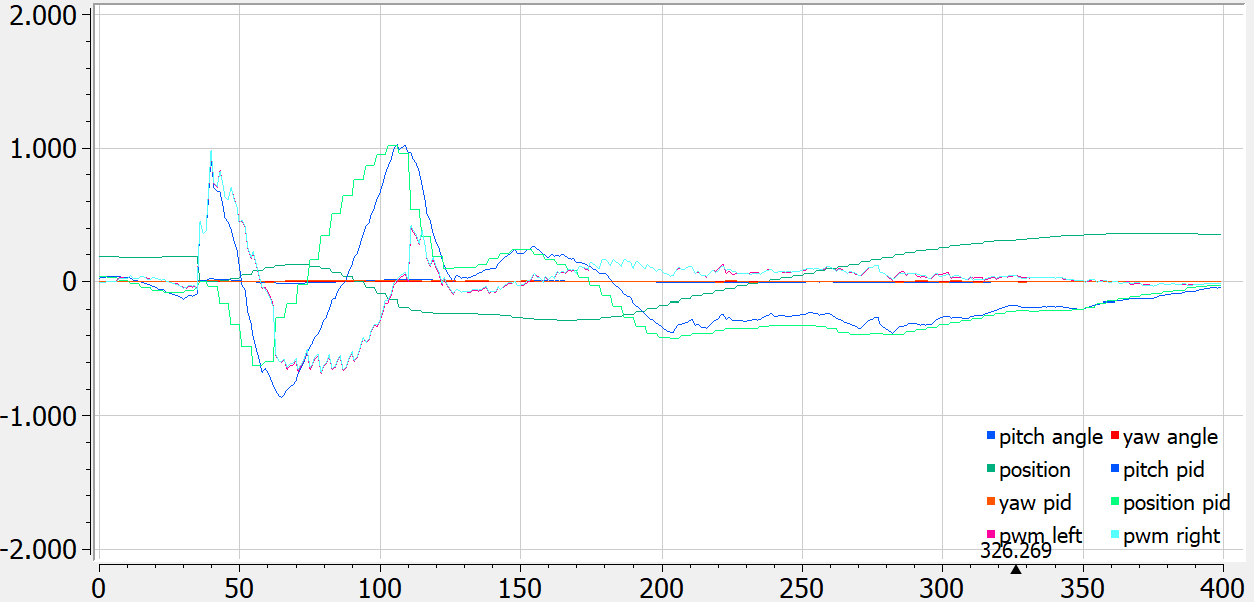
\includegraphics[width=0.8\linewidth]{assets/final_pid.png}
	\caption{The final control system individual output values recorded at baud rate of 115200.}
	\label{fig:final_pid}
\end{figure}


\begin{figure}[h]
	\centering
	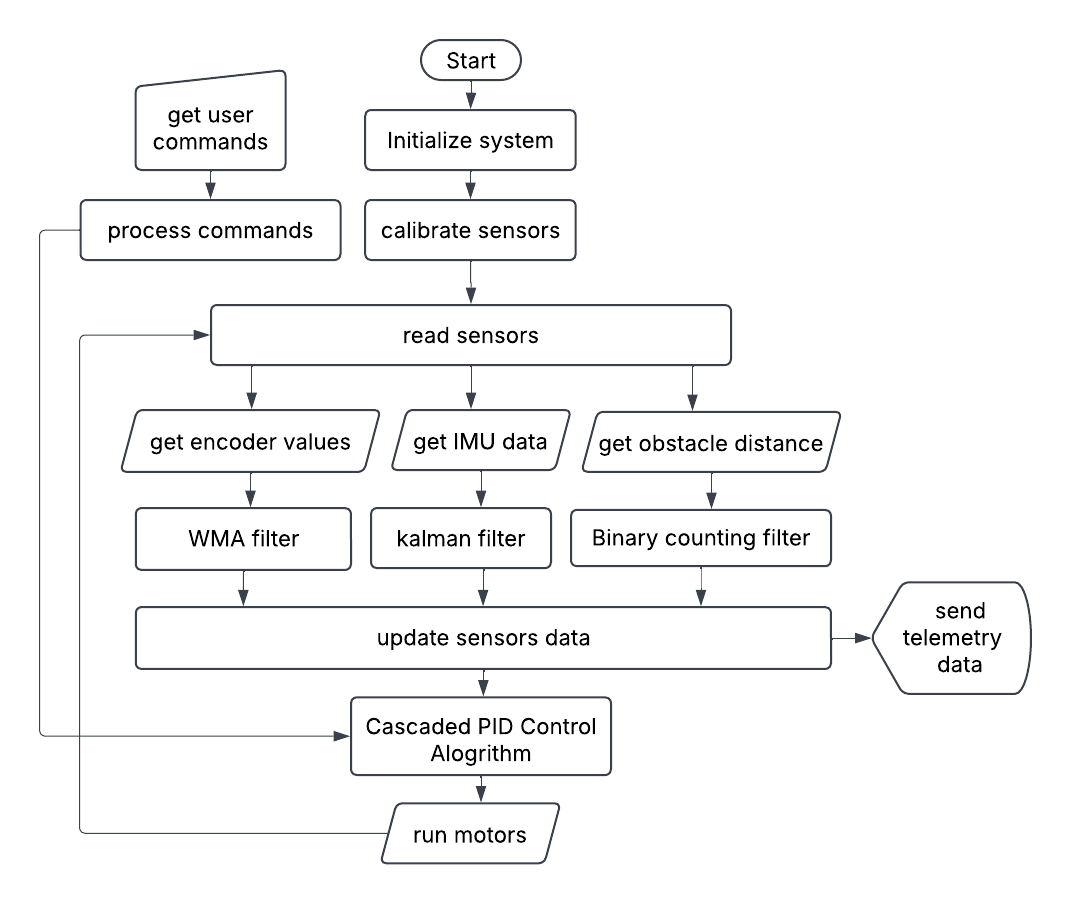
\includegraphics[width=0.8\linewidth]{assets/code_overview_flowchart.png}
	\caption{System operational flowchart for self-balancing mobile base.}
	\label{fig:code-overview-flowchart}
\end{figure}
